\section{Implementation} \label{sec:Implementation}

The initial MVP was designed with slight differences from the design outlined
in chapter \ref{sec:AnalysisAndDesign}. The most visible one is the fact that
what is mainly the Mediator pattern
(\cite[][Ch.~9,~Location~3594]{nikolov2016scala}) was used in order to
implement the dialogue between the presentation and other layers using a
feature similar to the MVC architecture. Normally, this type of architecture is
implemented in order to make sure that multiple views can refer to the same
core functionality (or model) without actually implementing that functionality
themselves, which allows the view to be responsible for presentation and the
model for liaising with the business logic through a controller. This also
allows the controller to update multiple existing views based on what input was
received from one view (\cite[][p.~381]{bennett2010object}). The difference in
the implementation for this project is that this last feature, essentially, was
not implemented. However, a mechanism was put in place which could allow for
this to happen.

In the implementation used for this project, the components were segregated
into packages and sub-packages. Each sub-package has been implemented so that
it does not have any knowledge of the super package, but rather exposes and
depends on interfaces which exist within itself. The super- (or outer)
packages, then, implement the interfaces of the sub-packages, which allows them
to interact with the sub-package components. The diagram below (Figure
\ref{fig:PresentationMVC}) illustrates this using the interaction between the
\texttt{InteractionMediator}, \texttt{SwingAmbassador} and \texttt{swing}
sub-package of the \texttt{presentation} package:

\begin{figure}[ht!]
  \begin{center}
    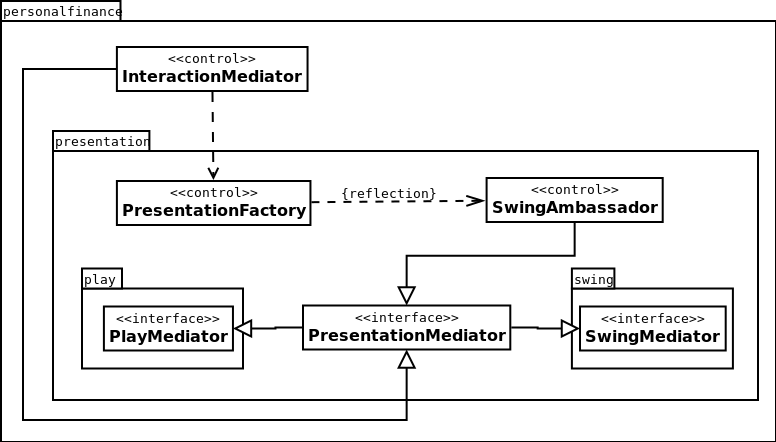
\includegraphics[width=15cm]{contents/img/Package_Diagram_-_Presentation_MVC.png}
  \end{center}
  \caption{}
  \label{fig:PresentationMVC}
\end{figure}
\FloatBarrier



In order to preserve encapsulation, specifically for the \texttt{swing}
package, only the \texttt{MainWindow} controller and \texttt{SwingMediator}
interface are exposed to the outside world, with the first having a constructor
dependency on the latter. This means that, in order to interact with the
components of the package, any external classes will need to implement the
\texttt{SwingMediator} interface. This is also useful if the
\texttt{presentation.swing} package is to be extracted and used as a library in
another code, and also leaves room for the \emph{Adaptor} pattern
(\cite[][p.~139]{gamma1995design}), if it needs to interact with other objects which do not
necessarily implement the interface upon which it depends.

One feature also noticeable in Figure \ref{fig:PresentationMVC} is the fact the
\texttt{personalfinance} package is unaware of which implementation of the view
it is interacting with. The \emph{Factory Method} pattern implemented on
\texttt{PresentationFactory}, which uses reflection to determine what
implementation to deliver, allows for the view itself to be decided with the
use of an external \texttt{.properties} file. This allows for the actual
dependency to change without the code having to be recompiled, which introduces
flexibility to the application. The \texttt{play} package is only a placeholder
at this point, as due to time constraints it was not possible to actually
implement it, but it is there to exemplify how the project can be further
extended.

\subsection{Scala Case Classes and the Prototype Design Pattern} \label{sec:Reflections.ScalaCaseClasses}
One of the benefits of Scala are its case classes. Not just are they very
useful for pattern matching, but also come with a few perks such as the
\texttt{copy()} method. This method allows for the class to be copied with some
or all its members modified. It could be said that it is a language-native
implementation of the \emph{Prototype Design Pattern}
(\cite[][Ch.~6,~Location~2461]{nikolov2016scala}), and throughout the
implementation and testing stage it proved to be a useful feature.

One of its many utilisations in this project can be seen in the
\texttt{Transaction} class, as one of the tools used to add entries to a
\texttt{Category} without having to change the state of a specific instance --
more similar to what is done in the \emph{Functional Programming} paradigm:
{
  \small
  \lstinputlisting[
    language=Scala,
    firstline=32,
    lastline=38,
    caption={
      extract of the \texttt{Transaction} class showing the \texttt{copy()}
      method in action
    }
  ]{../code/src/main/scala/personalfinance/businesslogic/transaction/Transaction.scala}
}


\subsection{Presentation Layer} \label{sec:Implementation.Presentation}
In the presentation layer, for the first iteration, the \emph{Scala Swing}
package was used for building most its aspects. The package consists of Scala
wrappers for the \emph{Java Swing} package, and one of the reasons why it was
chosen was that, as with many other GUI packages, it already comes with an
implementation of the \emph{Observer Design Pattern}
(\cite[][p.~293]{gamma1995design}) in its capacity to react to events
(\cite[][p.~5]{maier2009scala};
\cite[][Ch.~9,~Location~3731]{nikolov2016scala}).

\begin{sloppypar}
  The application starts by implementing the \texttt{MainMenu} class, which
  extends the \texttt{SimpleSwingApplication} abstract class from the
  \texttt{scala.swing} package. The class has an implementation of a \emph{main
  method}, therefore it acts as an entry point for the application to run. It
  also contains a \texttt{MainFrame}, which is a Swing \texttt{Frame} -- ``a
  window containing arbitrary data''
  (\cite[][Ch.~34,~Section~34.1]{odersky2016scala})-- which switches off the
  application when closed. It also has implementations of other methods to
  allow the application to close gracefully
  (\cite[][p.~2~\&~3]{maier2009scala}), so with these aspects implemented, it
  allows development to be focused on functionality more relevant to the
  application's logic itself.
\end{sloppypar}


\subsection{Business Logic} \label{sec:Implementation.BusinessLogic}

\textbf{TODO: syntax highlighting for code listings}

\textbf{TODO: write about how using properties file is a good way to decide
otherwise static behaviour at runtime -- is this dependency injection?}

\textbf{TODO: Write about how one of the advantages of scala is how it tries to
enforce the Universal Access. For example, Arrays and Lists implement the
interface (which I think is Iterable) which allows the user to completely
ignore how the data is implemented and access both as lists}

\textbf{TODO: write about why Validator has an auxiliary method for type --
generics would affect the interface. The Validator was created as a trait in
the first place to allow for lesser coupling between the classes which need
validation}

\textbf{TODO: write about why I chose to do integration tests rather than unit}

\textbf{TODO: Read the lightbend guide
https://www.lightbend.com/lagom-framework to Scala and Microservices}

\textbf{TODO: see if the below still makes sense}
The constraints from \texttt{Transaction} and \texttt{Pattern} were implemented
in the business logic code as follows:
{
  \small
  \lstinputlisting[
    language=Scala,
    firstline=15,
    lastline=24,
    caption={
      method to validate \texttt{Transaction} entries
    },
    label=DescriptiveLabel
  ]{../code/src/main/scala/personalfinance/businesslogic/transaction/Transaction.scala}
}

{
  \small
  \lstinputlisting[
    language=Scala,
    firstline=4,
    lastline=16,
    caption={
      snippet of \texttt{Pattern} showing requirement for it to have at least one Category
    }
  ]{../code/src/main/scala/personalfinance/businesslogic/transaction/Patterns.scala}
}

As Fowler (\citeyear[][]{fowler1997analysis}), one of the classes should be
responsible for keeping track of the relationship. As seen above, it was
decided that each \texttt{Category} will keep track of its patterns, and this
will at the same time enforce the constraint at the application layer level.


\textbf{Classifier was implemented with longest matching prefix: patterns are
matched to the start of the description of every entry, starting from longest
pattern to the shortest. This is so that if there is, for example, a pattern
"Laptop for girlfriend" which would match to category "Gifts", and another
pattern "laptop", for category "personal equipment", then entries with the
description "Laptop for Girlfriend" would not be picked up by the shorter match
for laptop.}

\textbf{TODO: talk about the decision to create constructor dependencies to
traits rather than classes directly, as is the case with
\texttt{DateStringParser}}

\textbf{TODO: talk about choosing not to user the Builder pattern for the Entry
class as it would turn into boilerplate town}

\textbf{TODO: talk about the small amount of input validation due to the first
version being for a desktop app only, but that if a hosted version were to be
made available more validation would be added}

\textbf{TODO: talk about the decision to have single methods to commit to the
database one entry at a time, which was because the database is local and
because it gives more control over when something goes wrong, both for
debugging or informing the end user. In future iterations, though, the plan was
to use batch versions as exemplified here
https://docs.oracle.com/javase/tutorial/jdbc/basics/prepared.html}

\textbf{Explain decision to make dependencies only flow in one direction --
namely, towards the more specialised packages (aside from the dependencies on
pre-compiled libraries, such as java.util and the ones listed on sbt) -- so
that the specialised modules could be extracted and reused in a more modular
fashion. Explain also why the modules in the default package are implementing
all similar interfaces in the more specialised ones, so that changes in the
more specialised ones which could affect dependencies will also have to be
implemented at the higher level, thus causing the flow to be maintained. E.g.,
each package declares PropertiesLoader, and the default package.}

\textbf{But: this has not been tested yet. Some classes such as PropertiesLoader are
private to the personalfiance package. This means that external pacakges cannot
import it directly, but would it be indirectly imported as a dependency when
importing other classes? Also, does it matter, since the dependency is actually
in an interface which is later implemented by the personalfinance package?}

\textbf{Talk how the above is a risky move, since Scala's mixin composition has
this habit of picking up the implementation of the last trait mixed into it, so
in this case you get PresentationMediator inheriting form SwingMediator and
then PlayMediator -- although both are traits, this could cause problems in the
future if the Play one implements something which Swing doesn't, so basically
these traits must always be the exact same}

\textbf{talk about the reason why the presentation mediator's methods returning
Unit being because this way they can stay as implementation-agnostic regarding
the other layers as they possibly can, again thinking that the interface needs
to be able to change without the code being recompiled}

\subsection{The Bridge Pattern} \label{sec:Implementation.TheBridgePattern}
\textbf{TODO: review this. It all changed after the 20th of April}
The Bridge pattern allows for an abstraction and its implementation to be
decoupled, so that both can vary independently
(\cite[][Ch.~7,Location~2699]{nikolov2016scala}). In this project, the bridge
pattern can be seen implemented in the \emph{presentation} and
\emph{persistence} layers. In the first, the \texttt{Presentation} class is
linked to the \texttt{PresentationBridge} trait by aggregation. The
\texttt{Swing} class implements this trait and refers to the \emph{swing}
package for the implementation. This was done so that the implementation of the
\emph{presentation} layer can change easily at runtime -- for example, if there
are a hosted and a portable version of the application, the first which runs on
a web framework and the latter with a desktop package such as Swing, the same
application can be implemented to both without the code having to be
recompiled.

Another feature which facilitates this is the fact that the clients -- the
\texttt{Presentation} class -- uses a combination of a
\texttt{java.util.Properties} object and \emph{reflection} to determine which
implementation it will run. This will also aid the above goal of having the
behaviour of the application change without it having to be recompiled.


\subsection{The Strategy Pattern} \label{sec:Implementation.TheStrategyPattern}

Thanks to Scala's mixin traits, the Strategy Pattern was implemented
successfully in the \texttt{PresentationMediator} class with only a few lines
of code. What happens here is that the combination of the Strategy and Factory
patterns are allow enough flexibility that the more specialised packages do not
have to depend on the packages which envelop it -- within the
\texttt{presentation} package there is a \texttt{swing} package and a
placeholder \texttt{play} package for the front-end implementations. So long as
the outer packages implement the interfaces for each specialised package, 

\subsection{Algebraic Data Types and the Value Object Pattern} \label{sec:Implementation.ADTAndValueObject}

Throughout the code, examples of Algebraic Data Types can be seen. These appear
in the form of sealed traits and case objects, and are normally used when
instances need to be passed around as values, but also contain information
which will be relevant to the code. Examples of these can be found in the
\texttt{ConnectionType} hierarchy, where the number of possible instances for
each case class would classify the trait and its subtypes as \emph{Product
Types} (\cite[][p.~411]{wampler2015programming}). The code listing below
illustrates this:

{
  \small
  \lstinputlisting[
    language=Scala,
    caption={
      extract of the \texttt{ConnectionType} hierarchy showing the case classes
      used as value objects
    }
  ]{../code/src/main/scala/personalfinance/persistence/connections/ConnectionType.scala}
}

Algebraic data types could be said to be the natural implementation of the
Value Object design pattern. This pattern is used widely for comparison of
objects not by their identities, but rather by their values. They consist of
small, immutable objects, and the instances of the case classes can be
classified as just those (\cite[][Ch.~8,~Location~3068]{nikolov2016scala}).
